\chapter{Introduction} \label{chap:Introduction}

In times where infectious disease outbreaks become more frequent and sometimes even reach global appearance, unpredictable effects on humans, wildlife and whole ecosystems are inevitable \autocite{schmeller_biodiversity_2020}. Growing human population and persisting poverty has harmful impact on the biodiversity and results in degradation of natural habitats and more frequent human-wildlife contacts  \autocite{schmeller_biodiversity_2020}. Therefore, increasing numbers of zoonoses, transfers of animal pathogens on humans, arise and are a major driving force in pathogen emergence on humans in recent decades \autocite{jones_global_2008}. Most of the human pathogens emerging lately are of animal origin, indeed, up to 75\% \autocite{woolhouse_risk_2001}. Well-known examples of zoonoses are avian and swine flu \gls{HIV}, ebola, \gls{MERS} and \gls{SARS} including the current circulating COVID-19 \autocite{van_reeth_avian_2007, sharp_origins_2011, suwantarat_risks_2015, verity_estimates_2020}.

While zoonoses can be of viral, bacterial and parasitic nature, emergences of higher magnitude, like the mentioned well-known examples, are often linked back to viral infections \autocite{woolhouse_risk_2001}. Harmfulness of viral infections can be diverse, ranging from mostly no sign of infection in the natural hosts to very severe symptoms or death in accidental hosts \autocite{wahlgren_influenza_2011}. High variety in host circulation and transmission ways from such natural or intermediate hosts onto humans, with long infectious periods without symptoms and high transmission pace have a high risk of pandemic events \autocite{jamison_disease_2017}. A prominent virus detected in a variety of hosts and known for reoccurring local and global outbreaks in the past is \gls{IAV}, member of the \textit{Orthomyoxoviridae} family and also commonly known as flu \autocite{wahlgren_influenza_2011}. Analysis indicate a 1\% chance of a pandemic with millions of influenza deaths every year and is, therefore, the pathogen most likely to be responsible for a sudden severe pandemic \autocite{jamison_disease_2017}. 

In humans, infection by \gls{IAV} affects the epithelial cells and leukocytes in is the upper respiratory tract \autocite{julkunen_inflammatory_2000}. General symptoms like fever, cough and headache characterize the infection \autocite{julkunen_inflammatory_2000}. In some cases complications can occur resulting in primary viral pneumonia or secondary bacterial pneumonia by bacterial infection \autocite{julkunen_inflammatory_2000}. By contact to tissue of the respiratory tract, the virus particles of \gls{IAV}, called virions, enter the cells \autocite{julkunen_inflammatory_2000, cann_principles_2016}.  Virions contain 



Segments \autocite{eisfeld_at_2015}

\begin{figure}
    \centering
    %\begin{adjustbox}{minipage=\dimexpr\textwidth-2\fboxsep-2\fboxrule,fbox}
    \begin{subfigure}[b]{0.475\textwidth}
        \caption[\textit{Alphainfluenzavirus}]{\textbf{\textit{Alphainfluenzavirus}}}
        \label{subfig:Influenza_A}
        \includegraphics[width=\textwidth]{Graphics/Influenza_A.pdf}
    \end{subfigure}
    \hfill
    \begin{subfigure}[b]{0.475\textwidth}
        \caption[\textit{Betainfluenzavirus}]{\textbf{\textit{Betainfluenzavirus}}}
        \label{subfig:Influenza_B}
        \includegraphics[width=\textwidth]{Graphics/Influenza_B.pdf}
    \end{subfigure}
    %\end{adjustbox}
    \caption[\textit{Orthomyxoviridae}]{\textbf{\textit{Orthomyxoviridae}.} .}
    \label{fig:Orthomyxoviridae}
\end{figure}


Present day research indicate mallards \textit{(Anas platyrhynchos)} as main reservoir and natural host of \glspl{LPAIV} \autocite{jourdain_influenza_2010}. 


% hierarchical clustering \autocite{gower_minimum_1969}. 

% \blindtext

% \begin{figure}
%     \centering
%     %\begin{adjustbox}{minipage=\dimexpr\textwidth-2\fboxsep-2\fboxrule,fbox}
%     \begin{subfigure}[b]{0.475\textwidth}
%         \caption[Compactness]{\textbf{Compactness}}
%         \label{subfig:Compactness}            
%         \includegraphics[width=\textwidth]{Graphics/Compactness.pdf}
%     \end{subfigure}
%     \hfill
%     \begin{subfigure}[b]{0.475\textwidth}
%         \caption[Connectedness]{\textbf{Connectedness}}
%         \label{subfig:Connectedness}            
%         \includegraphics[width=\textwidth]{Graphics/Connectedness.pdf}
%     \end{subfigure}
%     %\end{adjustbox}
%     \caption[Clustering Methods]{\textbf{Clustering Methods.} .}
%     \label{fig:Methods}
% \end{figure}

% \blindtext

% \begin{figure}
%     \centering
%     %\begin{adjustbox}{minipage=\dimexpr\textwidth-2\fboxsep-2\fboxrule,fbox}
%     \begin{subfigure}[b]{0.475\textwidth}
%         \caption[Euclidean]{\textbf{Euclidean}}
%         \label{subfig:Euclidean}
%         \includegraphics[width=\textwidth]{Graphics/Euclidean.pdf}
%     \end{subfigure}
%     \hfill
%     \begin{subfigure}[b]{0.475\textwidth}
%         \caption[Cosine]{\textbf{Cosine}}
%         \label{subfig:Cosinus}            
%         \includegraphics[width=\textwidth]{Graphics/Cosinus.pdf}
%     \end{subfigure}
%     %\end{adjustbox}
%     \caption[Distance Measuring Methods]{\textbf{Distance Measuring Methods.} .}
%     \label{fig:Distance}
% \end{figure}

% \blindtext

% % \begin{fequation}[!hbt]
% %     \begin{empheq}[box=\fbox]{alignat* = -1}
% %         &xL &&&&+zL &&\longrightarrow xL &&&&+zH\\
% %         &xM &&+yL &&+zH &&\longrightarrow xM &&+yL &&+zL\\
% %         &xM &&+yM &&+zL &&\longrightarrow xM &&+yM &&+zH\\
% %         &xH &&+yL &&+zH &&\longrightarrow xH &&+yL &&+zL\\
% %         &xH &&+yM &&+zH &&\longrightarrow xH &&+yM &&+zL\\
% %         & &&\hphantom{++}yH &&+zL &&\longrightarrow &&\hphantom{++}yH &&+zH
% %     \end{empheq}
% %     \caption[]{\textbf{.}}
% %     \label{gl:8.2}
% % \end{fequation}

% \textbf{Normalization with max-norm:} 
% %is the normalization so that the l2 norm of a vector is 1 !!!!!

% \begin{empheq}{alignat = -1}
%     \hat{\mathbf{x}} &= \frac{\mathbf{x}}{\Vert\mathbf{x}\Vert_{\text{max}}}
% \end{empheq}

% \begin{empheq}{alignat = -1}
%     \Vert\hat{\mathbf{x}}\Vert_{\text{max}} &= 1
% \end{empheq}

% \textbf{Cosinus similarity:}

% \begin{empheq}{alignat = -1}
%     %&\cos\angle(\mathbf{x}, \mathbf{y}) &&= \frac{\mathbf{x}^\top\mathbf{y}}{\Vert\mathbf{x}\Vert \cdot \Vert\mathbf{y}\Vert}
%     &\cos(\Theta) &&= \frac{\mathbf{x}^\top\mathbf{y}}{\Vert\mathbf{x}\Vert \cdot \Vert\mathbf{y}\Vert}
% \end{empheq}

% \textbf{cosinus distance}

% \begin{empheq}{alignat = -1}
%     %&d(\mathbf{x},\mathbf{y}) &&= 1 - \cos\angle(\mathbf{x}, \mathbf{y})
%     &d(\mathbf{x},\mathbf{y}) &&= 1 - \cos(\Theta)
% \end{empheq}

% \textbf{euclidean distance:}

% \begin{empheq}{alignat = -1}
%     &d(\mathbf{x},\mathbf{y}) &&= \Vert\mathbf{x} - \mathbf{y}\Vert_2
% \end{empheq}

% %gute anzahl cluster mit nennen 50-100 suoer bzw <100
% %außerdem erwartet, dass ansatzweise wie subtype bei H und N